\section{Fonctionnement}
\paragraph{}
Ce projet est issu d'un besoin de supervision et d'audit sécurité système dans le réseau d'une entreprise d'aujourd'hui.
\subsection{Objectif}
\paragraph{}
Octopus a pour objectif d'être un outil d'administration réseau répondant à un besoin de gestion d'un parc informatique par un administrateur réseau. 
\paragraph{}
Le nom du projet vient de la pieuvre qui a une tête qui contient le cerveau et qui dirige le reste de son corps, et les nombreuses tentacules de celle-ci qui ne sont que l'éxécution des commandes du cerveau (« brain ») et fait remonter des informations à ce « brain ». 
L'idée est donc d'avoir un point de contrôle central pour l'administrateur qui est le « brain » et ensuite chaque poste du parc informatique correspond à une tentacule (« tentacle »). 
\paragraph{}
L'outil d'administration que nous proposons permet de connaître en temps réel le statut de connexion au réseau des postes distants et de pouvoir lancer des scripts sur ces machines distantes. Les résultats des scripts sont disponibles sur le poste d'administration. Nous pouvons alors connaître à un moment donné l'état d'utilisation du disque dur d'un poste, l'état des processus lancé sur un autre poste, … La gestion du serveur est faite à travers une interface Web accessible avec des identifiants pour l'administrateur. Depuis cette interface, nous pouvons gérer le parc, ajouter de nouvelles machines, voir l'état du parc, commander l'éxécution de scripts sur les hôtes distants.
\paragraph{}
Le serveur est multi-client et permet donc la gestion d'un parc informatique important. L'administrateur peut créer des scripts afin de ne gérer que les informations dont il juge importante pour son parc. Un échantillon de script de base est installé par défaut dans le package client.


\subsection{Algorithme}

\paragraph{}
Dans un premier temps, nous avons travaillé sur un algorithme de notre solution afin de montrer le fonctionnement et les points-clés de celle-ci.
\paragraph{}
Les fonctionnalités maitre/esclave que présente Octopus Supervisor sont :
\begin{itemize}
 \item Ajout de nouveaux esclaves
 \item Gestion des esclaves
 \item Envoi de scripts aux esclaves
 \item Réception et stockage de résultats de scripts sur le serveur
\end{itemize}

\begin{figure}[!h]
    \centering
    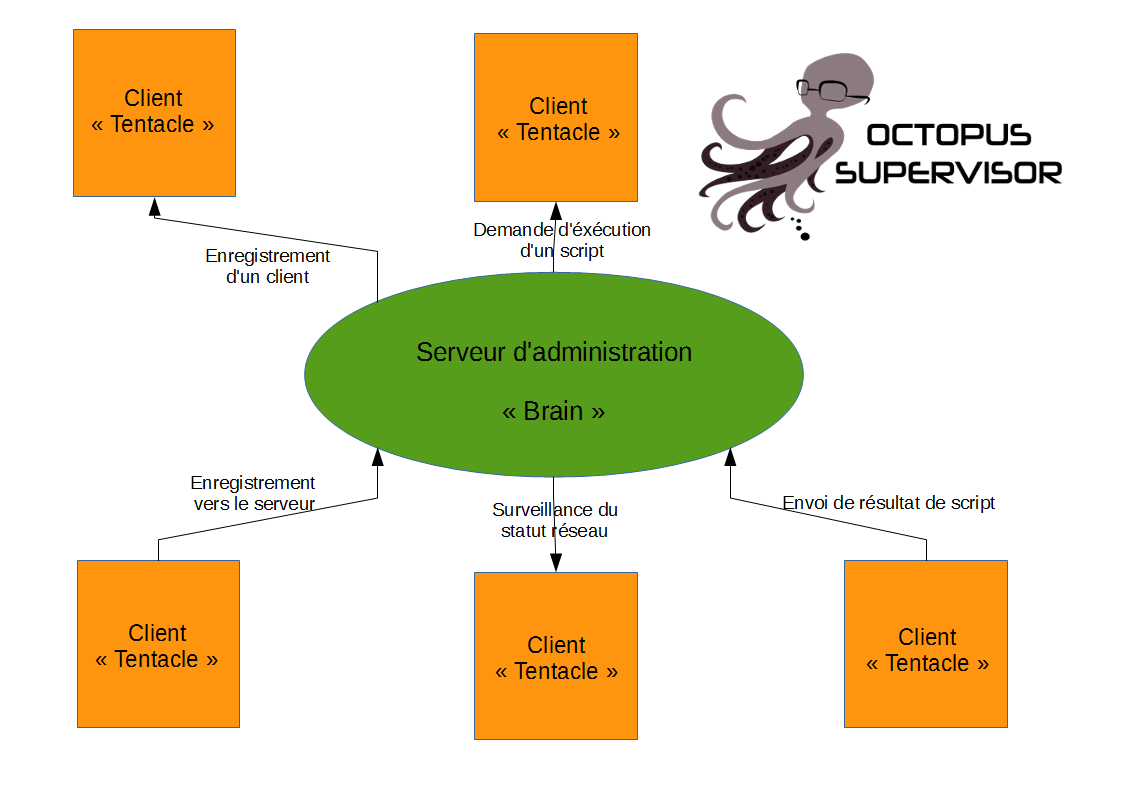
\includegraphics[width=\textwidth]{img/algo_general.png}
    \caption{Algorithme général de fonctionnement de Octopus Supervisor}
\end{figure}

\paragraph{}
Ci-dessous, un algorithme explicite techniquement le fonctionnement général de Octopus Supervisor.
\paragraph{}
Les deux entités maitre et esclave communiquent sur le réseau grâce à leur adresse IP et un port défini suivant le type de communication. Lors de l'enregistrement d'un client, le serveur est réceptif sur le port 6000. Si le client n'a pas de serveur spécifié lors de son lancement, il va attendre une communication sur le port 7000 de la part d'un serveur.
\begin{figure}[!h]
    \centering
    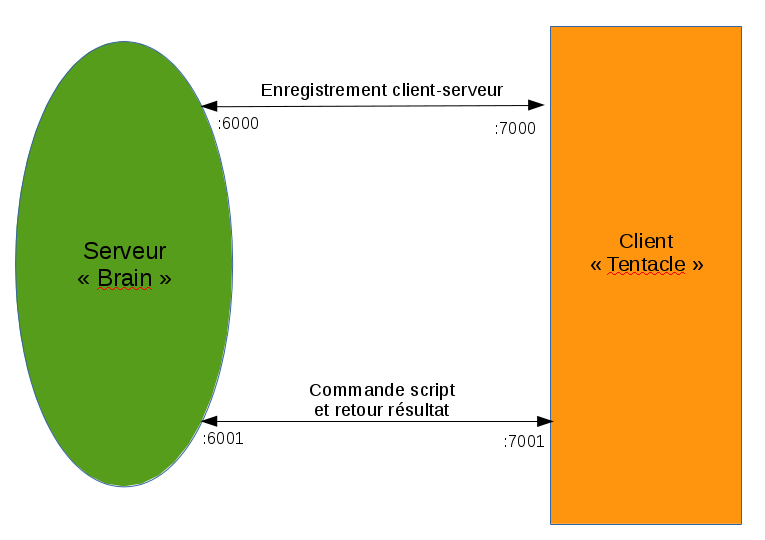
\includegraphics[width=\textwidth,height=9cm,keepaspectratio=true]{img/fct.png}
    \caption{Fonctionnement}
\end{figure}
